\chapter*{Tareas}
\addcontentsline{toc}{chapter}{Tareas}


\section*{Papers importantes de explorar en la evolucion de la tesis}

\begin{enumerate}
        \item dos papers adicionales para mirarlos. En algun momento serán necesario leerlos por ahora solo los dejo presentes. Si puede darle un mirada rapida, aqui puede usar IA
    \url{https://iopscience.iop.org/article/10.3847/1538-4357/abaef9/pdf}
    \url{https://iopscience.iop.org/article/10.3847/1538-4357/ac17e9/pdf}
\end{enumerate}


\newpage

Papers obligatorios para analizar:

\begin{enumerate}

    \item Metodologia:
    \begin{itemize}
    \item
    KINEMATIC TREATMENT OF CORONAL MASS EJECTION EVOLUTION IN THE SOLAR WIND
    \item
    Direct First Parker Solar Probe Observation of the Interaction of Two Successive Interplanetary Coronal Mass Ejections in 2020 November
    \item
    An Analytical Model of Interplanetary Coronal Mass Ejection Interactions
    \item
    Morphological and Kinematic Evolution of Three Interacting Coronal Mass Ejections of 2011 February 13-15
    \item
    Analyses of the Evolution and Interaction of Multiple Coronal Mass Ejections and Their Shocks in July 2012
    \item
    The Interaction Between Coronal Mass Ejections and Streamers: A Statistical View over 15 Years (1996 - 2010)
    \item
    The Interaction of Two Coronal Mass Ejections: Influence of Relative Orientation
    \item
    Characteristics of Kinematics of a Coronal Mass Ejection during the 2010 August 1 CME-CME Interaction Event
    \item
    SWASTi-CME: A Physics-based Model to Study Coronal Mass Ejection Evolution and
Its Interaction with Solar Wind
\item
A STATISTICAL STUDY OF MAIN AND RESIDUAL ACCELERATIONS
OF CORONAL MASS EJECTIONS
\end{itemize}

    \item Cálculos \& Discusión
    \begin{itemize}
        \item Successive Interacting Coronal Mass Ejections: How to Create a Perfect Storm
    \item Interaction of coronal mass ejections and the solar wind. A force analysis

    \end{itemize}
    

    \item Discusion: 
    \begin{itemize}
        \item
    Deriving the Interaction Point between a Coronal Mass Ejection and High-speed Stream: A Case Study
    \item
    Interaction of a coronal mass ejection and a stream interaction region: A case study
    \item
    Interaction between Two Coronal Mass Ejections in the 2013 May 22 Large Solar Energetic Particle Event
    \item
    The Role of Coronal Mass Ejection Interactions in the Acceleration of Solar Energetic Particle Events
    \item
    Do Interacting Coronal Mass Ejections Play a Role in Solar Energetic Particle Events?
    \item
    Radio Signatures of Coronal Mass Ejection Interaction: Coronal Mass Ejection Cannibalism?
    \end{itemize}
    

    \item Conclusiones
    \begin{itemize}
         \item
    Does the direct interaction between coronal mass ejections play a role in the acceleration of solar energetic particles?

    \item Numerical Simulation of the Interaction of Two Coronal Mass Ejections from Sun to Earth
    \end{itemize}
   
\end{enumerate}

\begin{figure}[H]
    \centering
    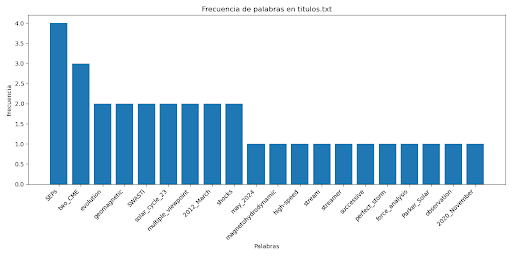
\includegraphics[width=0.9\linewidth]{Imagenes Mein/Frecuencia palabras.png}
    \caption{Frecuencia de palabras en paper \textcite{gonzalez-esparza-2004}.}
\end{figure}